\documentclass[11pt]{book}
\usepackage{palatino}
\usepackage{amsfonts,amsmath,amssymb}
% \usepackage{graphicx}


\ifx\pdftexversion\undefined
    \usepackage[dvips]{graphicx}
\else
    \usepackage[pdftex]{graphicx}
    \usepackage{epstopdf}
    \epstopdfsetup{suffix=}
\fi


\begin{document}

%%%%%%%%%%%%%%%%%%%%%%%%%%%%%%%%%%%%%%%%
% Problem Set 5
%%%%%%%%%%%%%%%%%%%%%%%%%%%%%%%%%%%%%%%%

\pagestyle{empty}
{\noindent\bf Spring 2021 \hfill Ali Berra}
\vskip 16pt
\centerline{\bf University of Central Florida}
\centerline{\bf College of Business}
\vskip 16pt
\centerline{\bf QMB 6911}
\centerline{\bf Capstone Project in Business Analytics}
\vskip 10pt
\centerline{\bf Solutions:  Problem Set \#5}
\vskip 32pt
\noindent




\section{Used Trucks Data}

Begin with creating the variable age from the year variable, and taking in consideration that the data was gathered in 2020.

\subsection{Scatterplots of the data type, pau, pret, milage, damge, ror, and cost}

 
%
\begin{figure}[h!]
  \centering
  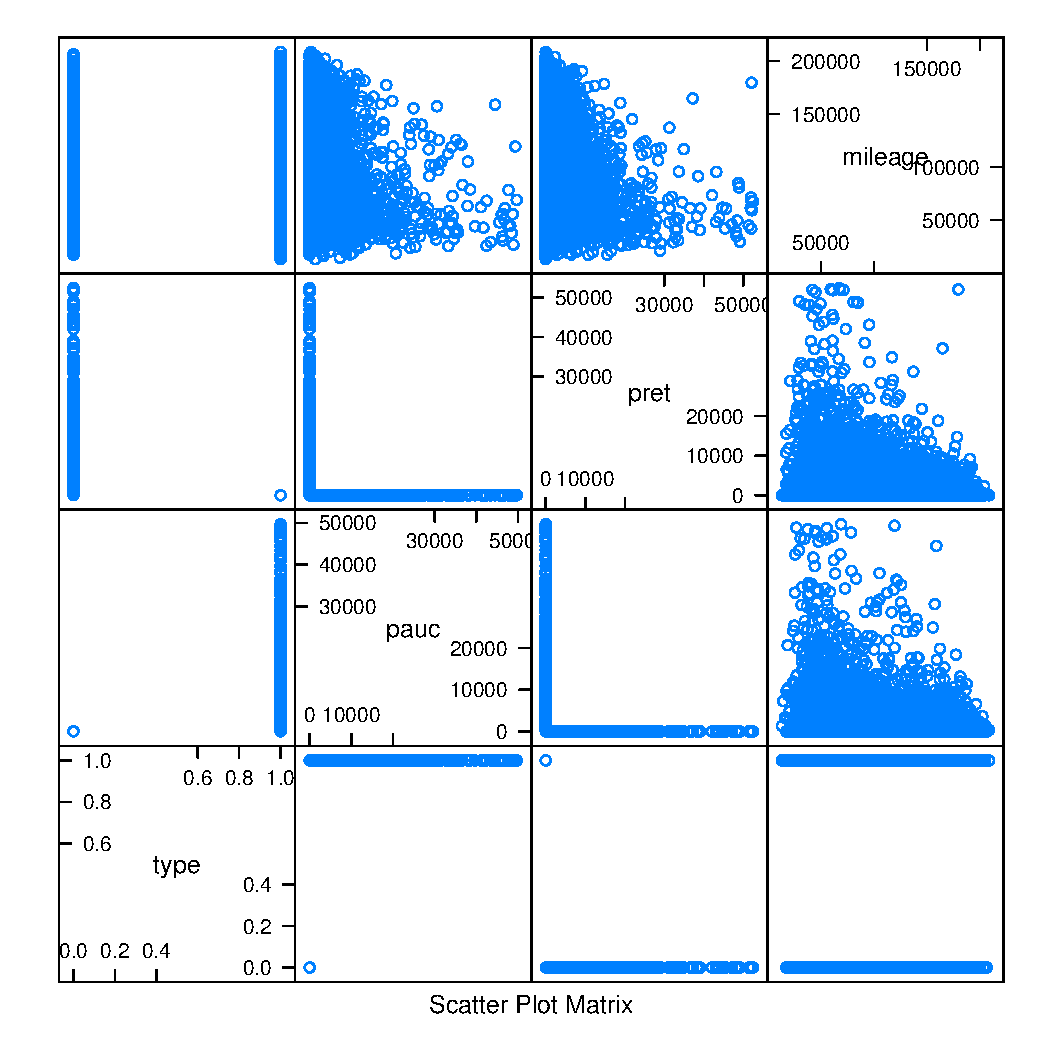
\includegraphics[scale = 0.5, keepaspectratio=true]{../Figures/slpom_num_only}
  \caption{matrix of scatterplots} \label{fig:splom_num_only}
\end{figure}
% .


\clearpage
\pagebreak
\subsection{considering differences bewtween the dealer and age}




\begin{figure}[h!]
  \centering
  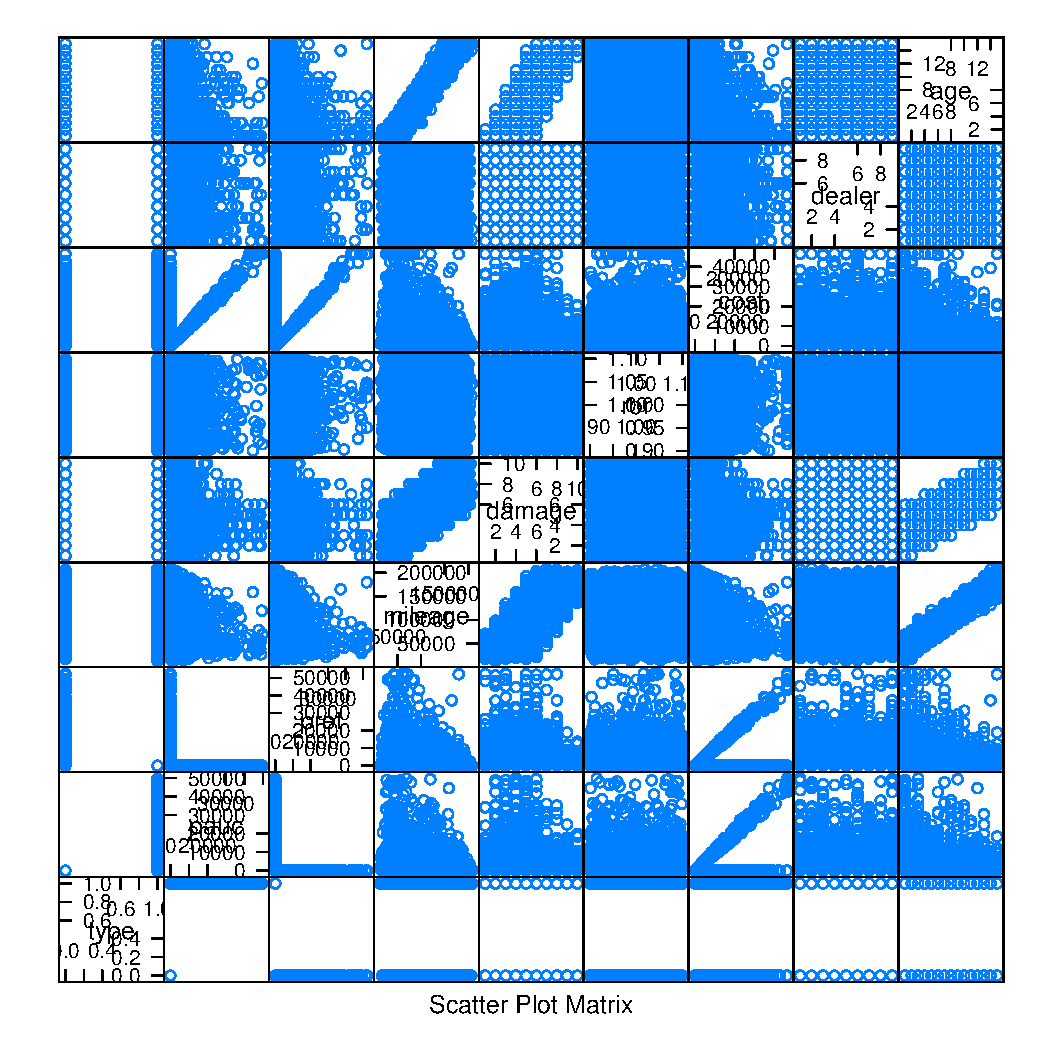
\includegraphics[scale = 0.5, keepaspectratio=true]{../Figures/slpom_with_cat}
  \caption{considering dealer and age} \label{fig:splom_with_cat}
\end{figure}


\clearpage
\pagebreak



\subsection*{cheking the relationshp between mileage and age }


Figure \ref{fig:age_mileage_plot} showing the relationship between mileage and age 


\begin{figure}[h!]
  \centering
  \includegraphics[scale = 0.5, keepaspectratio=true]{../Figures/age_mileage_plot}
  \caption{relationship between mileage and age} \label{fig:age_mileage_plot}
\end{figure}


\clearpage
\pagebreak

\subsection*{cheking the relationship between pret and age }




\begin{figure}[h!]
  \centering
  \includegraphics[scale = 0.5, keepaspectratio=true]{../Figures/pret_age_plot}
  \caption{comparing the relationship between retail price and age} \label{fig:pret_age_plot}
\end{figure}

\clearpage
\pagebreak



\subsection*{cheking the relationship between pauc and age }




\begin{figure}[h!]
  \centering
  \includegraphics[scale = 0.5, keepaspectratio=true]{../Figures/pauc_age_plot}
  \caption{comparing the relationship between auction price and age} \label{fig:pauct_age_plot}
\end{figure}







%%%%%%%%%%%%%%%%%%%%%%%%%%%%%%%%%%%%%%%%
\end{document}
%%%%%%%%%%%%%%%%%%%%%%%%%%%%%%%%%%%%%%%%
